\documentclass{article}
\usepackage[utf8]{inputenc}
\usepackage[italian]{babel}
\usepackage{amsmath}
\usepackage{amssymb}
\usepackage{siunitx}
\usepackage{tabularray}
\usepackage{graphicx}
\usepackage{float}
\usepackage{minted}
\usepackage[page]{appendix}
\newcommand*{\diam}{\varnothing}
\newcommand*{\best}[1]{{#1}_\text{best}}
\newcommand*{\bestp}[1]{{\left(#1\right)}_\text{best}}
\newcommand*{\pbest}[1]{\left({#1}_\text{best}\right)}
\newcommand*{\pbestp}[1]{\left({\left(#1\right)}_\text{best}\right)}
\newcommand*{\errrel}[1]{\frac{\delta #1}{{#1}_\text{best}}}
\title{
    Laboratorio di Fisica 1\\
    R6: Misura dei calori specifici di materiali ignoti
}
\author{Gruppo 17: Bergamaschi Riccardo, Graiani Elia, Moglia Simone}
\date{8/11/2023 – 15/11/2023}
\makeindex
\begin{document}

\maketitle

\begin{abstract}
    Il gruppo di lavoro ha misurato il calore specifico di tre solidi distinti
    per risalirne alla natura.
\end{abstract}

\section{Materiali e strumenti di misura utilizzati}
\begin{center}
    \begin{tblr}{ |Q[l,m]|Q[c,m]|Q[c,m]|Q[c,m]| }
        \hline
        \textbf{Strumento di misura} & \textbf{\:\:\:\:\:Soglia\:\:\:\:\:} & \textbf{Portata} & \textbf{Sensibilità} \\
        \hline
        Termometro digitale & $\qty{00}{\degree C}$ & $\qty{00}{\degree C}$ & $\qty{0.1}{\degree C}$ \\
        % \hline[dashed]
        % Termometro a mercurio & $\qty{0.1}{\degree C}?$ & $\qty{100}{\degree C}?$ & $\qty{0.1}{\degree C}?$ \\
        \hline[dashed]
        Barometro & $\qty{0}{hPa}?$ & $\qty{14000}{hPa}$ & $\qty{1}{hPa}$ \\
        \hline[dashed]
        Cilindro graduato & $\qty{1}{mL}?$ & $\qty{100}{mL}$ & $\qty{1}{mL}$ \\
        \hline[dashed]
        Bilancia di precisione & $\qty{0.50}{g}$ & $\qty{4100.00}{g}$ & $\qty{0.01}{g}$ \\
        \hline
        \hline
        \textbf{Altro} & \SetCell[c=3]{l} \textbf{Descrizione/Note} \\
        \hline
        Calorimetro & \SetCell[c=3]{l} {Isolato termicamente, quasi adiabatico.} \\
        \hline[dashed]
        {Fornelletto e pentolino} & \SetCell[c=3]{l} {Per scaldare acqua e campioni.} \\
        \hline[dashed]
        Tre campioni solidi & \SetCell[c=3]{l} {Li chiameremo $A$, $B$ e $C$.} \\
        \hline
    \end{tblr}
\end{center}

\section{Misurazione della massa equivalente}
    
\subsection{Esperienza e procedimento di misura}
    
\begin{enumerate}
    \item
        Versiamo in un cilindro graduato $\qty{100}{mL}$ di acqua distillata e, dopo
        averla pesata con la bilancia di precisione, la mettiamo a scaldare in un pentolino.
    \item
        Ripetiamo il passaggio precedente, ma invece di scaldarla, questa volta
        versiamo l'acqua a temperatura ambiente nel calorimetro.
        
    \emph{
        \textbf{Osservazione.}È meglio che le masse si equivalgano, e che la loro
        somma sia uguale all'acqua che utilizzeremo nella seconda parte dell'esperimento,
        in modo che il calorimetro si bagni allo stesso modo.
        }
        
    \item
        Quando l'acqua raggiunge lo stato di ebollizione, che corrisponde circa a 
        $\qty{100}{\degree C}$, la versiamo nel calorimetro e mescoliamo lentamente
        per evitare che l'acqua calda resti in alto. Il termometro digitale ci
        darà il valore della temperatura in funzione del tempo.
\end{enumerate}
        
\subsection{Analisi dei dati raccolti e conclusioni}
Per le leggi della termodinamica noi sappiamo che:
    \[
        m_\text{calda} c_\text{acqua} (T_\text{calda}-T_\text{eq}) =
        (m_\text{fredda} c_\text{acqua} + C_\text{calorimetro})(T_\text{eq}-T_\text{fredda})
    \]

Invece che misurare $C_\text{calorimetro}$ in $\unit{J\per K}$, possiamo considerare a
quanta acqua equivale il calorimetro dal punto di vista termico, ovvero la quantità di
acqua che assorbirebbe lo stesso calore del calorimetro. Quindi:
    \[
        m_\text{calda} (T_\text{calda}-T_\text{eq}) =
        (m_\text{fredda} + m_\text{equiv})(T_\text{eq}-T_\text{fredda})
    \]

    \emph{
        \textbf{Osservazione.} La massa equivalente ($m_\text{equiv}$) ci da anche un idea di
        quanto il calorimetro disturbi la misura.
        }


\subsection{Scritto}
    Dobbiamo misurare il calore specifico degli oggetti a noi dati. Il calore
    specifico $c$ è la quantità di calore necessaria ad aumentare di $\qty{1}{K}$ una
    quantità unitaria di massa ($\qty{1}{kg}$) e cambia da sostanza a sostanza.
    Se abbiamo oggetti composti da più materiali possiamo utilizzare come grandezza,
    anche se contiene meno informazioni, la capacità termica $C$, ovvero il calore
    necessario ad un oggetto per innalzare la sua temperatura di $\qty{1}{K}$.

    L'equazione che dobbiamo tenere presente è $Q=m c \Delta T$.

    Per determinare il calore specifico di un oggetto dobbiamo conoscerne la massa,
    che si misura con la bilancia, lo sbalzo termico, che si misura con i due
    termometri, uno a mercurio e uno digitale, e il calore assorbito o ceduto dal
    corpo, che, però, non è misurabile in modo immediato.
    Si può misurare in un sistema isolato termicamente, come un calorimetro adiabatico
    dove mettiamo il corpo a contatto con un'altro corpo (per esempio una massa
    d'acqua) di cui conosciamo i valori precedentemente descritti.
    Mettendo due corpi, uno caldo e uno freddo, a contatto termico in un sistema
    isolato e in cui non viene svolto lavoro meccanico, sappiamo che il corpo caldo
    cederà calore al corpo freddo fino al raggiungimento di una temperatura di
    equilibrio e che $\Delta Q_\text{ced}=-\Delta Q_\text{ass}$ (conservazione dell'energia).

    Se noi scaldiamo uno dei solidi  % TODO: quali solidi?
    nell'acqua bollente, ovvero in corrispondenza
    della transizione di quest'ultima da stato liquido ad aeriforme, tutto il sistema
    è a $\qty{100}{\degree C}$, salvo correzioni dovute alla pressione diversa da $\qty{1}{atm}$.
    L'acqua da noi utilizzata è distillata ($c=\qty{4186}{J \per kg\,K}$)
    Quando accendiamo il fornelletto, per farlo scaldare più velocemente e assicurarci
    di essere in stato di ebollizione, regoliamo la temperatura della piastra a
    $T>\qty{100}{\degree C}$.
    Quando il cilindretto raggiunge la temperatura di 100°C lo mettiamo nel calorimetro,
    nel quale si troverà acqua a temperatura ambiente, ma prima di fare questo
    trasferimento facciamo partire la misura della temperatura. Chiuso il calorimetro,
    mescoliamo (per evitare che l'acqua calda resti in alto).

    \[
        m_\text{met} c_\text{met} (T_\text{caldo}-T_\text{eq}) =
        c_\text{acqua} m_\text{acqua} (T_\text{eq}-T_\text{fredda})
    \]

    "Il calorimetro è abbastanza adiabatico e questo lo valuterete nell'ultima parte
    dell'esperimento."

    \[
        m_\text{met} c_\text{met} (T_\text{caldo}-T_\text{eq}) =
        (c_\text{acqua} m_\text{acqua} + C_\text{calorimetro}) (T_\text{eq}-T_\text{fredda})
    \]. Questa è la seconda parte dell'esperimento.

    È necessaria una prima parte dell'esperimento per misurare $C_\text{calorimetro}$
    Prendiamo due masse d'acqua, una fredda da mettere nel calorimetro ed una da
    scaldare nel pentolino. È meglio che le masse si equivalgano, e che la loro
    somma sia uguale all'acqua che utilizzeremo nella seconda parte, in modo che
    il calorimetro si bagni allo stesso modo.
    Raggiunti i 100°C, versiamo l'acqua calda nel calorimetro. Allora:

    \[
        m_\text{calda} c_\text{acqua} (T_\text{calda}-T_\text{eq}) =
        (m_\text{fredda} c_\text{acqua} + C_\text{calorimetro})(T_\text{eq}-T_\text{fredda})
    \]

    Invece che misurare $C_\text{calorimetro}$ in $\unit{J\per K}$, possiamo considerare a quanta acqua equivale
    il calorimetro dal punto di vista termico, ovvero la quantità di acqua che assorbirebbe lo
    stesso calore del calorimetro.

    \[
        m_\text{calda} (T_\text{calda}-T_\text{eq}) =
        (m_\text{fredda} + m_\text{equiv})(T_\text{eq}-T_\text{fredda})
    \]

    \emph{
        \textbf{Osservazione.} La massa equivalente ($m_\text{equiv}$) ci da anche un idea di
        quanto il calorimetro disturbi la misura.
    }

    Una volta ottenuto questo valore, possiamo calcolare i calori specifici dei metalli
    di cui sono composti i cilindretti.

    Come ultima cosa misureremo la discesa esponenziale della temperatura dell'acqua
    dentro al calorimetro e in particolare il suo tempo caratteristico, ovvero la quantità
    di tempo $\tau$ che impiega l'acqua all'interno del calorimetro ad abbassare la sua
    temperatura di $(T_0 - T_\text{amb})e$ volte.

    La legge che segue questa discesa è: \[(T-T_\text{amb.})=(T_0-T_\text{amb.}) e^{-t/\tau}\]

    Il parametro $\tau$ descrive quanto bene il calorimetro trattenga il calore
    (quindi sia adiabatico). Per misurarlo abbiamo scaldato $\qty{200}{g}$ d'acqua, che abbiamo
    poi lasciato raffreddare nel calorimetro in partenza vuoto, registrandone la $T$.

    L'equazione della regressione lineare che abbiamo utilizzato è:
    \[\ln(T-T_\text{amb.})=\ln(T_0-T_\text{amb.})-\frac{1}{\tau}t\]



\section{Processo di Bernoulli}
\subsection{Materiali e strumenti di misura utilizzati}
\begin{center}
    \begin{tblr}{ |Q[l,m]|Q[c,m]| }
        \hline
        \textbf{Materiali} & \textbf{Descrizione/Note} \\
        \hline
        Sei dadi & Di colori diversi, per poterli identificare facilmente \\
        \hline
        Calcolatore & Computer portatile\footnotemark \\
        \hline
    \end{tblr}
\end{center}
\footnotetext{Intel core i5 gen 7 dual-core \qty{1,6}{GHz}}

\subsection{Dati sperimentali}
Eseguiamo 400 lanci di sei dadi distinti\footnote{Li distinguiamo in base al colore},
registrandone tutti i risultati.
Per ogni possibile risultato\footnote{
    \emph{Notazione.} Per noi $0\in\mathbb{N}$.
} $s\in\left[1;6\right]\cap\mathbb{N}$, possiamo così
definire una variabile aleatoria $x_s\in\left[0;6\right]\cap\mathbb{N}$ come il
numero di dadi, fra i sei lanciati, con risultato pari ad $s$.
Il lancio dei sei dadi è un processo di Bernoulli; di conseguenza,
la distribuzione di probabilità di $x_s$ è data da:
\[
    p \left(x_s=k\right) =
        \binom{6}{k}
        \left(\frac{1}{6}\right)^k
        \left(\frac{5}{6}\right)^{6-k}
        \qquad\forall k\in\left[0;6\right]\cap\mathbb{N}
\]
Di seguito riportiamo gli istogrammi dei dati così raccolti, assieme ai valori attesi,
dedotti dalla distribuzione teorica.

\begin{figure*}
    \caption{...}
\end{figure*}

\subsubsection*{Onestà dei dadi}
Avendo segnato tutti i risultati di ogni dado, possiamo inoltre stimare se i dadi che
abbiamo utilizzato sono truccati o meno. Infatti, su un dado onesto ci aspettiamo
che escano tutti i risultati possibili con equa probabilità. Di seguito riportiamo
gli istogrammi dei valori usciti su ogni dado.

\begin{figure*}
    \caption{...}
\end{figure*}

\subsection{Simulazione}
Tramite un programma da noi scritto e compilato\footnote{\emph{Vedi} Appendice 1},
simuliamo la stessa esperienza con $10^{12}$ lanci dei sei dadi al fine di
verificare la legge dei grandi numeri. Questa consiste nella tesi che, su un grande
numero di prove, i risultati si avvicinino ai valori attesi.

Di seguito riportiamo, in un istogramma, i risultati della simulazione.

\section{Processo di Poisson}
\subsection{Materiali e strumenti di misura utilizzati}
\begin{center}
    \begin{tblr}{ |Q[l,m]|Q[c,m]|Q[c,m]|Q[c,m]| }
        \hline
        \textbf{Strumento di misura} & \textbf{\:\:\:\:\:Soglia\:\:\:\:\:} & \textbf{Portata} & \textbf{Sensibilità} \\
        \hline
        {Contatore Geiger} & \qty{1}{conteggi \per s} & ??? & \qty{1}{conteggi \per s} \\
        \hline[dashed]
        Metro a nastro & \qty{0.1}{cm} & \qty{300.0}{cm} & \qty{0.1}{cm} \\
        \hline
        \hline
        \textbf{Altro} & \SetCell[c=3]{l} \textbf{Descrizione/Note} \\
        \hline
        {Sei dadi} & \SetCell[c=3]{l} {
            Usati per riprodurre un processo\\
            bernoulliano.
            } \\
            \hline[dashed]
            {Campione di Torio-232} & \SetCell[c=3]{l} {
                Usato per riprodurre un processo\\
                poissoniano.
            } \\
        \hline
    \end{tblr}
\end{center}


\subsection{Esperienza e procedimento di misura}
\begin{enumerate}
    \item Acceso e impostato adeguatamente il contatore Geiger, misuriamo per 5 diverse distanze
          tra contatore e campione il numero di raggi $\gamma_{ij}$ emessi da quest'ultimo in 3600 intervalli da un secondo.
    \item Direzionato il contatore dal verso opposto rispetto al campione, misuriamo il numero di raggi $\gamma_{amb}$ rilevabili che definiscono
          il fondo dei nostri dati.
\end{enumerate}

Fissato un sistema di riferimento solidale all'apparato di misura, con origine
nella posizione di partenza delle sferette e $\hat{x} = \hat{g}$, possiamo
scrivere la seguente legge del moto:
\[x(t) = \frac{1}{2}g t^2\]
Per ogni sferetta $i$, posto $x\left(\overline{t_i}\right) = d_0 - \frac{1}{2}\diam_i$,
la norma di $\vec{g}$ è ricavabile da:
\[
    g = \frac{2d_0 - \diam_i}{\left(\overline{t_i}\right)^2}
    % \best{g} = \frac{2\best{\left(d_0\right)} - \bestp{\diam_i}}
    %                 {\bestp{\overline{t_i}}^2}
    % \qquad\wedge\qquad
    % \errrel{g} = \frac{2\left(\delta d_0\right) - \delta \diam_i}
    %                   {2\best{\left(d_0\right)} - \bestp{\diam_i}}
    %            + 2\frac{\sigma_{\overline{t_i}}}{\overline{t_i}}
\]
dove determiniamo l'errore su $g$ propagando gli errori su $d_0,\diam_i$ e
$\overline{t_i}$, avendo posto
\[
    \delta\overline{t_i} =
    \sigma_{\overline{t_i}} =
    \frac{\sigma_{t_i}}{\sqrt{100}} =
    \frac{\sigma_{t_i}}{10}.
\]
\\

Di seguito riportiamo gli istogrammi dei tempi e i valori di $g$ così ottenuti.


\begin{figure}[H]
    %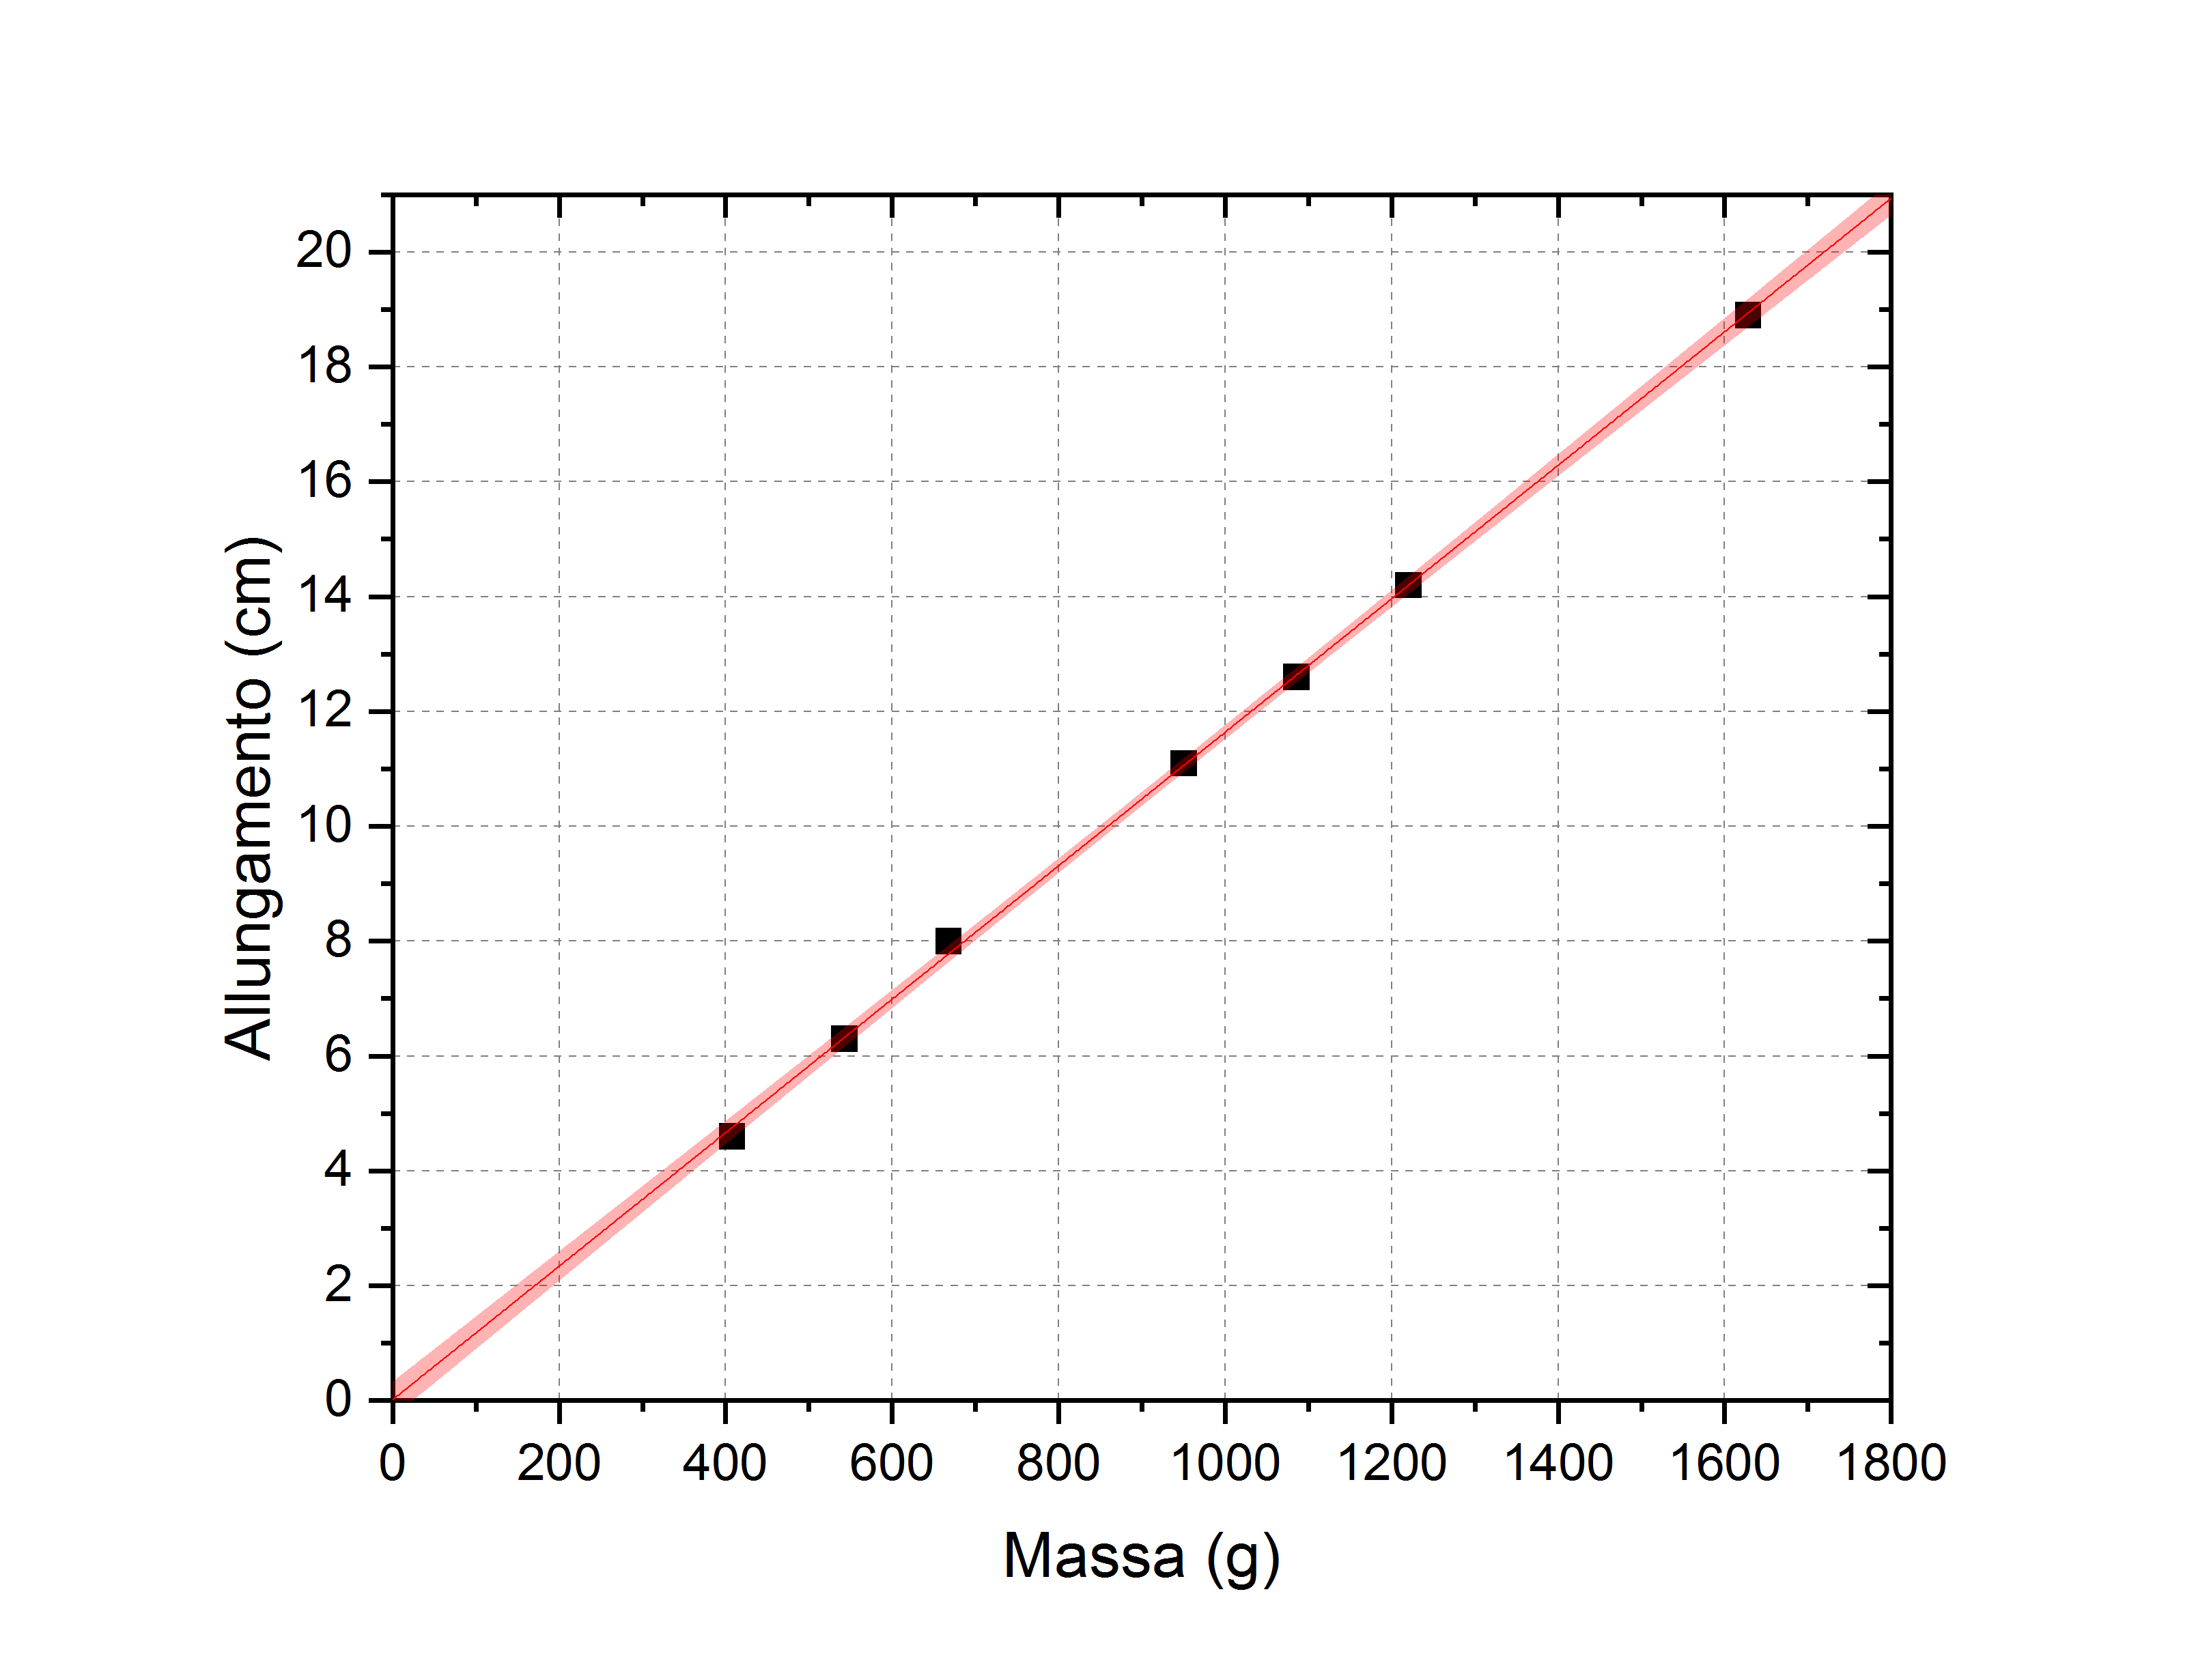
\includegraphics[trim={0 1.8cm 0 0},width=\textwidth]{SaticoReg.jpg}
    \caption{Istogrammi dei dati $t_1$ e $t_2$ raccolti}
\end{figure}
\begin{center}
    \begin{tblr}{ |Q[c,m]|Q[c,m]|Q[c,m]|Q[c,m]|Q[c,m]| }
        \hline
            $i$ &
            $\diam_i\:(\unit{mm})$ &
            $\overline{t_i}\:(\unit{ms})$ &
            $g\:(\unit{m\per s^2})$ &
            $\varepsilon$ \\
        \hline
        A & $24.63\pm0.01$ & $503.62\pm0.03$ & $9.83\pm0.02$ & $1.00$ \\
        \hline[dashed]
        B & $22.23\pm0.01$ & $503.91\pm0.03$ & $9.82\pm0.02$ & $0.93$ \\
        \hline
    \end{tblr}
\end{center}

\subsection{Esperienza sulla distribuzione di Poisson}
\begin{enumerate}
    \item Consideriamo la distanza tra i due fototraguardi e impostiamo i fotodiodi
          del contatore su A+B.
    \item Usando solo
    \begin{enumerate}
        \item Appeso il campione alla molla, allineiamo i due fototraguardi
              aiutandoci con la livella, in modo tale che possano rilevare
              le oscillazioni nel modo più accurato possibile;
        \item Tiriamo leggermente il campione verso il basso e poi lo rilasciamo,
              in modo che il sistema molla inizi a oscillare con direzione
              il più possibile parallela a $\vec{g}$;
        \item Attesa la stabilizzazione dell’oscillazione, avviamo
              l'acquisizione della misura di un tempo (20 periodi)
              $20T_i$.
        \item Ripetiamo molte volte (in tutto $N_{20T_i}$) i punti
              (b) e (c). In particolare, $N_{20T_A} = N_{20T_B} = 25$
              e $N_{20T_C} = N_{20T_{A+B}} = 30$.
    \end{enumerate}
    \item Infine, misuriamo con la bilancia, separatamente,
          la massa della molla $m_m$ e la massa del gancio $m_g$.
\end{enumerate}

Infatti, nel caso dinamico, il contributo di queste masse
\emph{non} si annulla; in particolare, la massa del gancio
contribuisce appieno (in quanto è solidale col grave),
mentre la massa della molla contribuisce per circa
$\frac{1}{3}$. La massa effettiva da considerare per ogni grave
sarà allora:
\[\best{\left(\left(m_\text{eff}\right)_i\right)} = \best{\left(m_i\right)} + \best{\left(m_g\right)} + \frac{1}{3}\best{\left(m_m\right)}\]
\[\delta \left(m_\text{eff}\right)_i = \delta m_i + \delta m_g + \frac{1}{3}\delta m_m\]

Di seguito sono riportate le distribuzioni dei dati raccolti:

\begin{figure}[H]
    %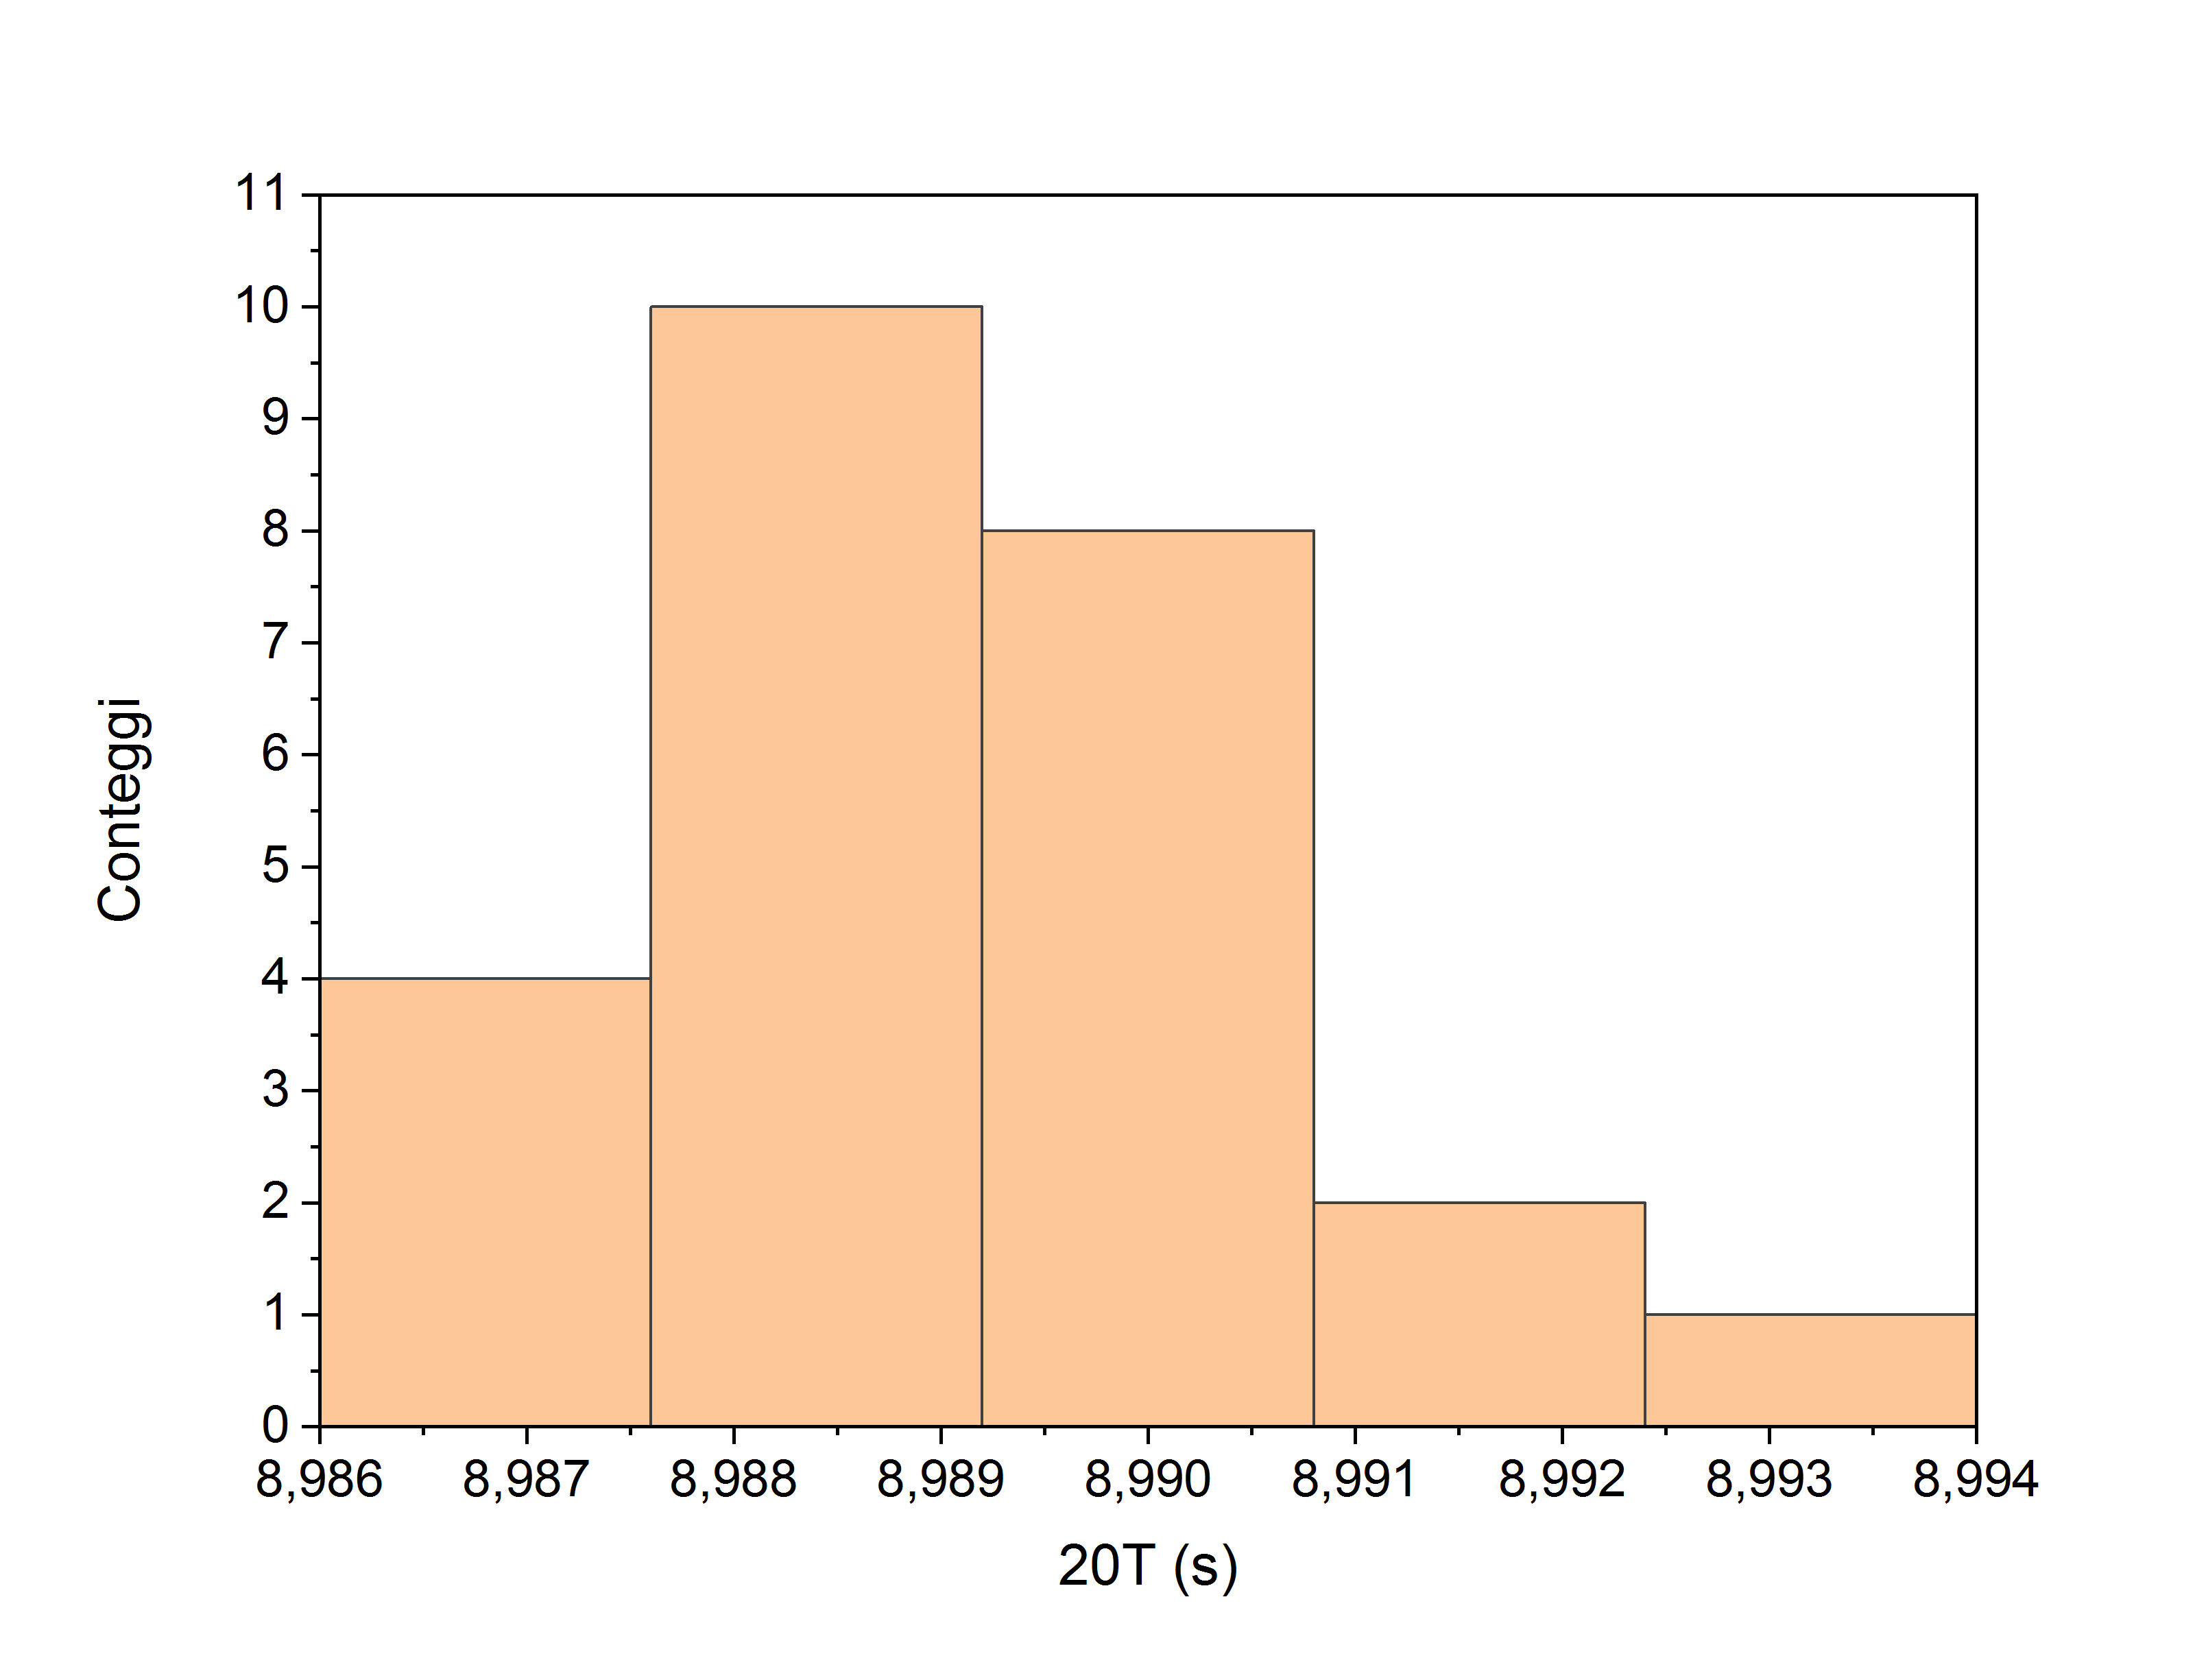
\includegraphics[trim={2cm 1.8cm .7cm 1.5cm},width=.5\textwidth]{Dinamico1.jpg}
    %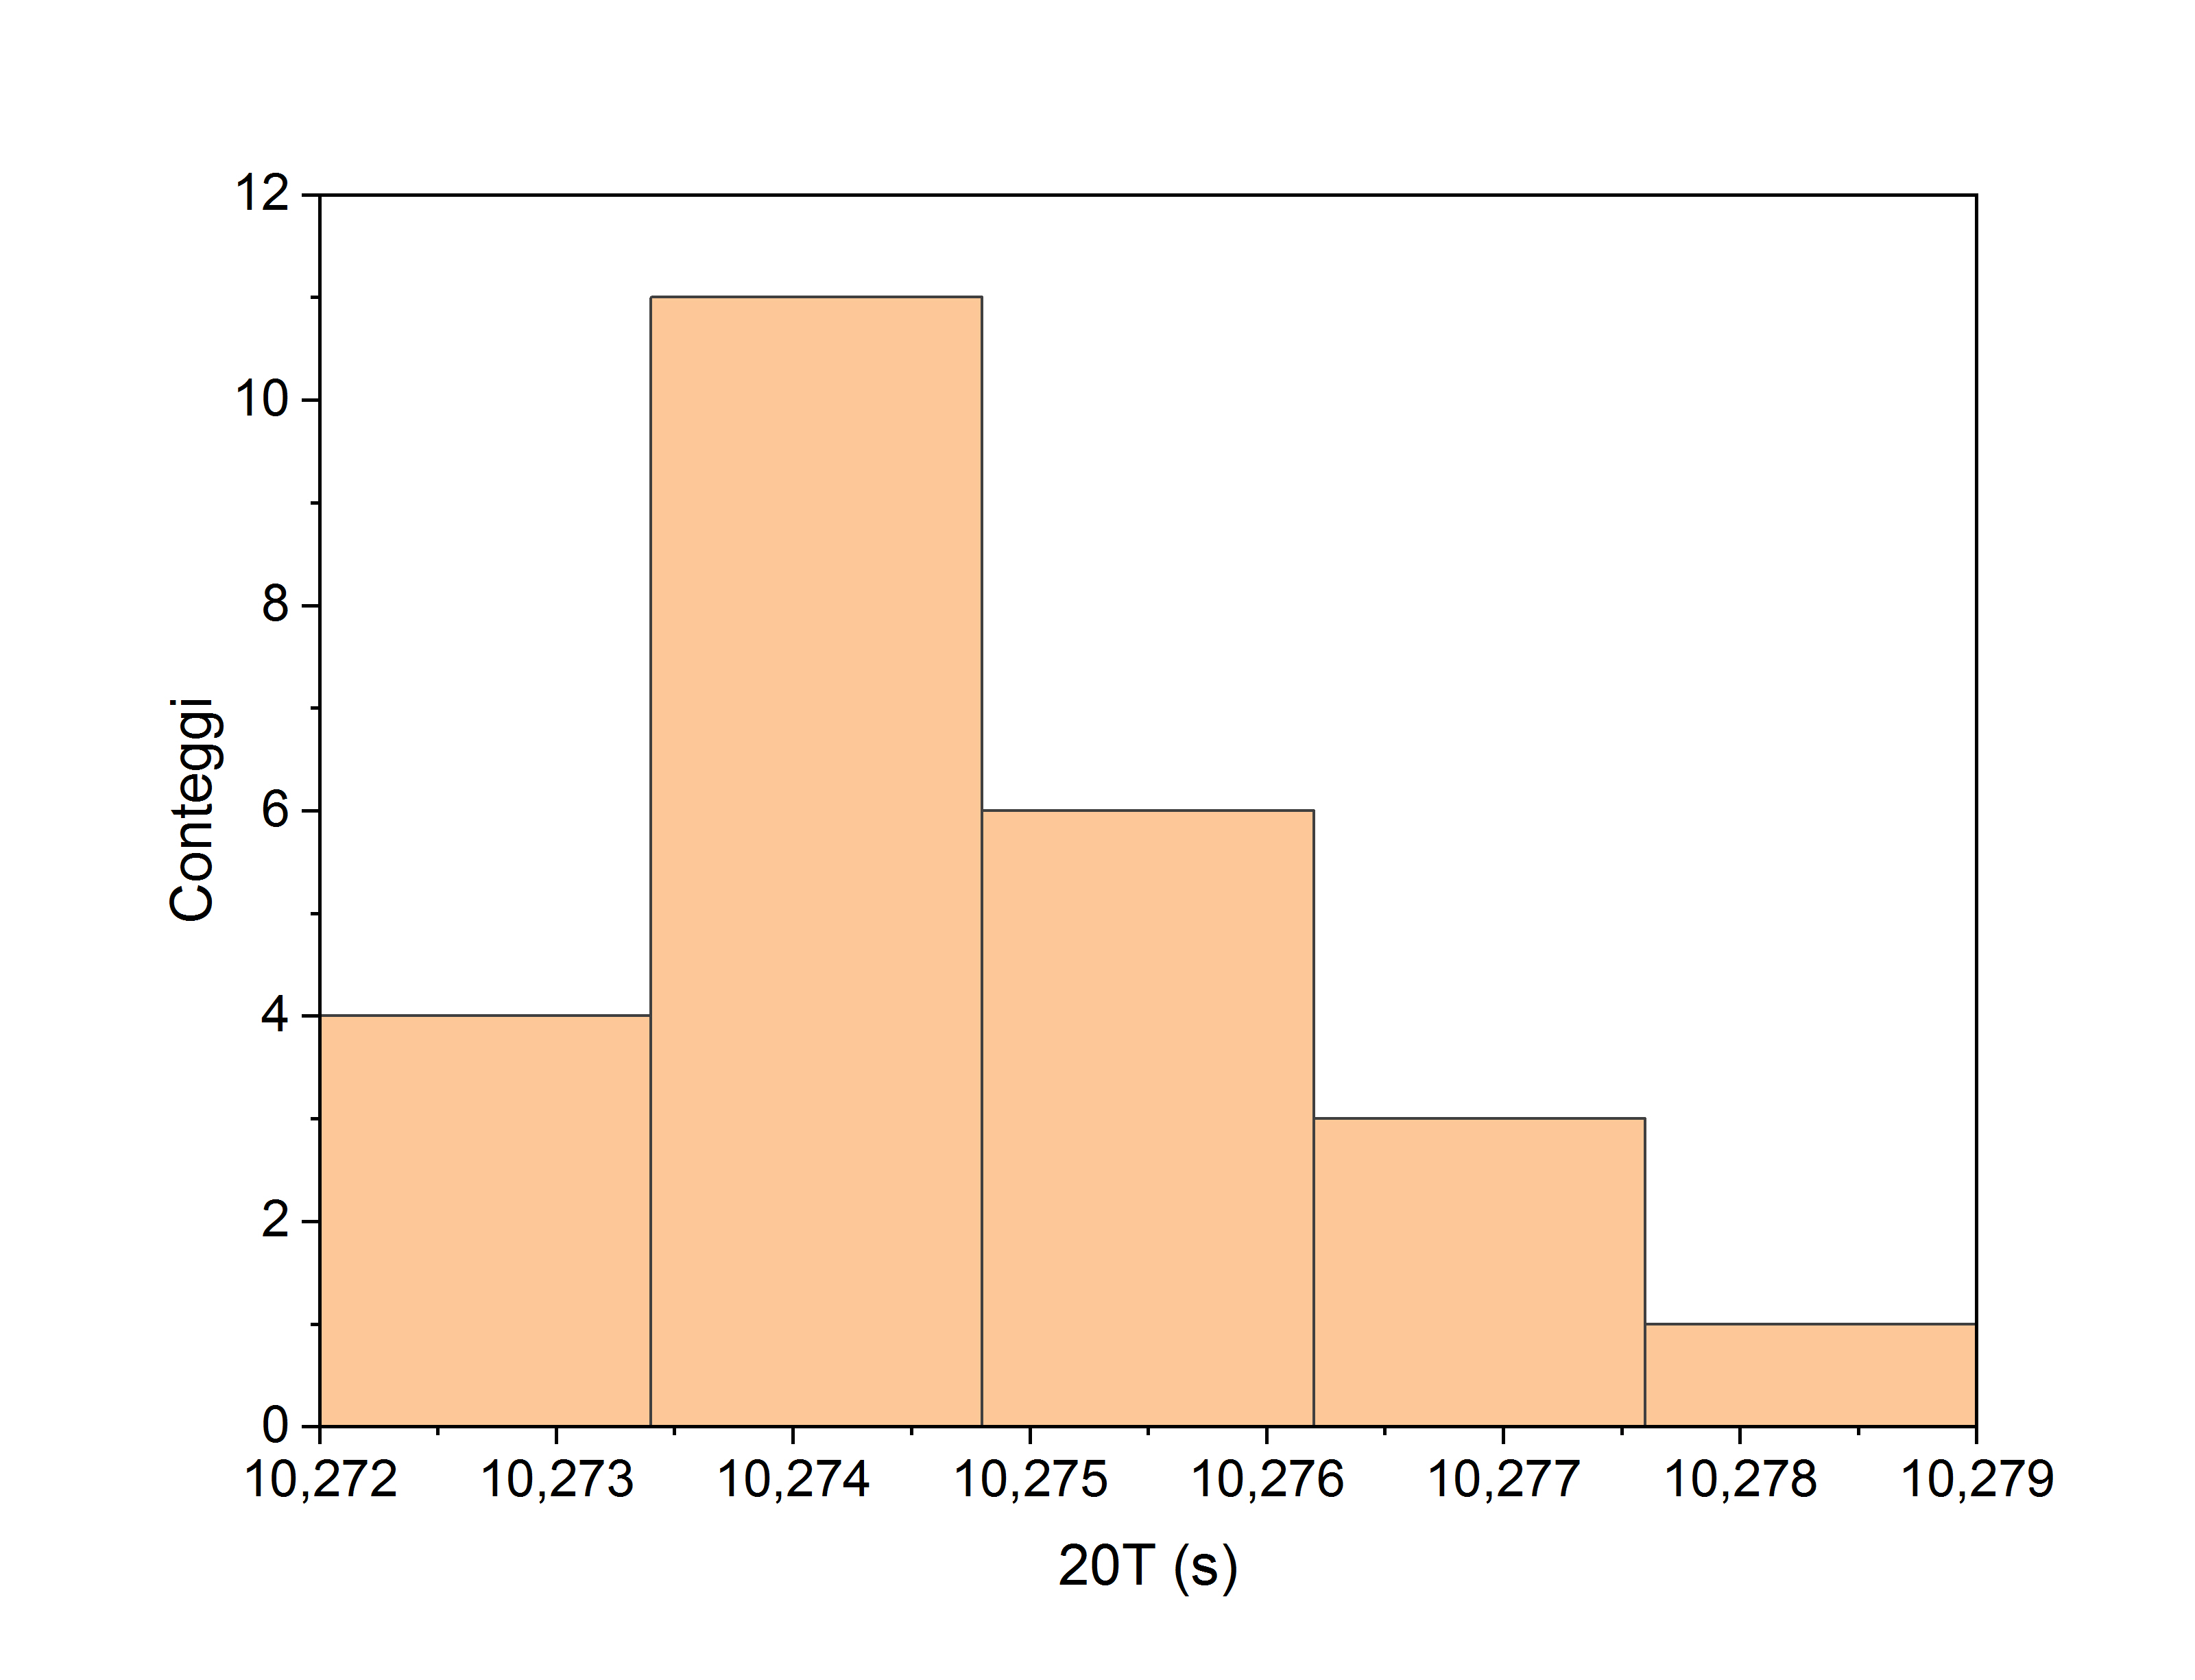
\includegraphics[trim={.7cm 1.8cm 2cm 1.5cm},width=.5\textwidth]{Dinamico2.jpg}
    \caption{Istogrammi dei periodi delle oscillazioni di $A$ e $B$}
\end{figure}\begin{figure}[H]
    %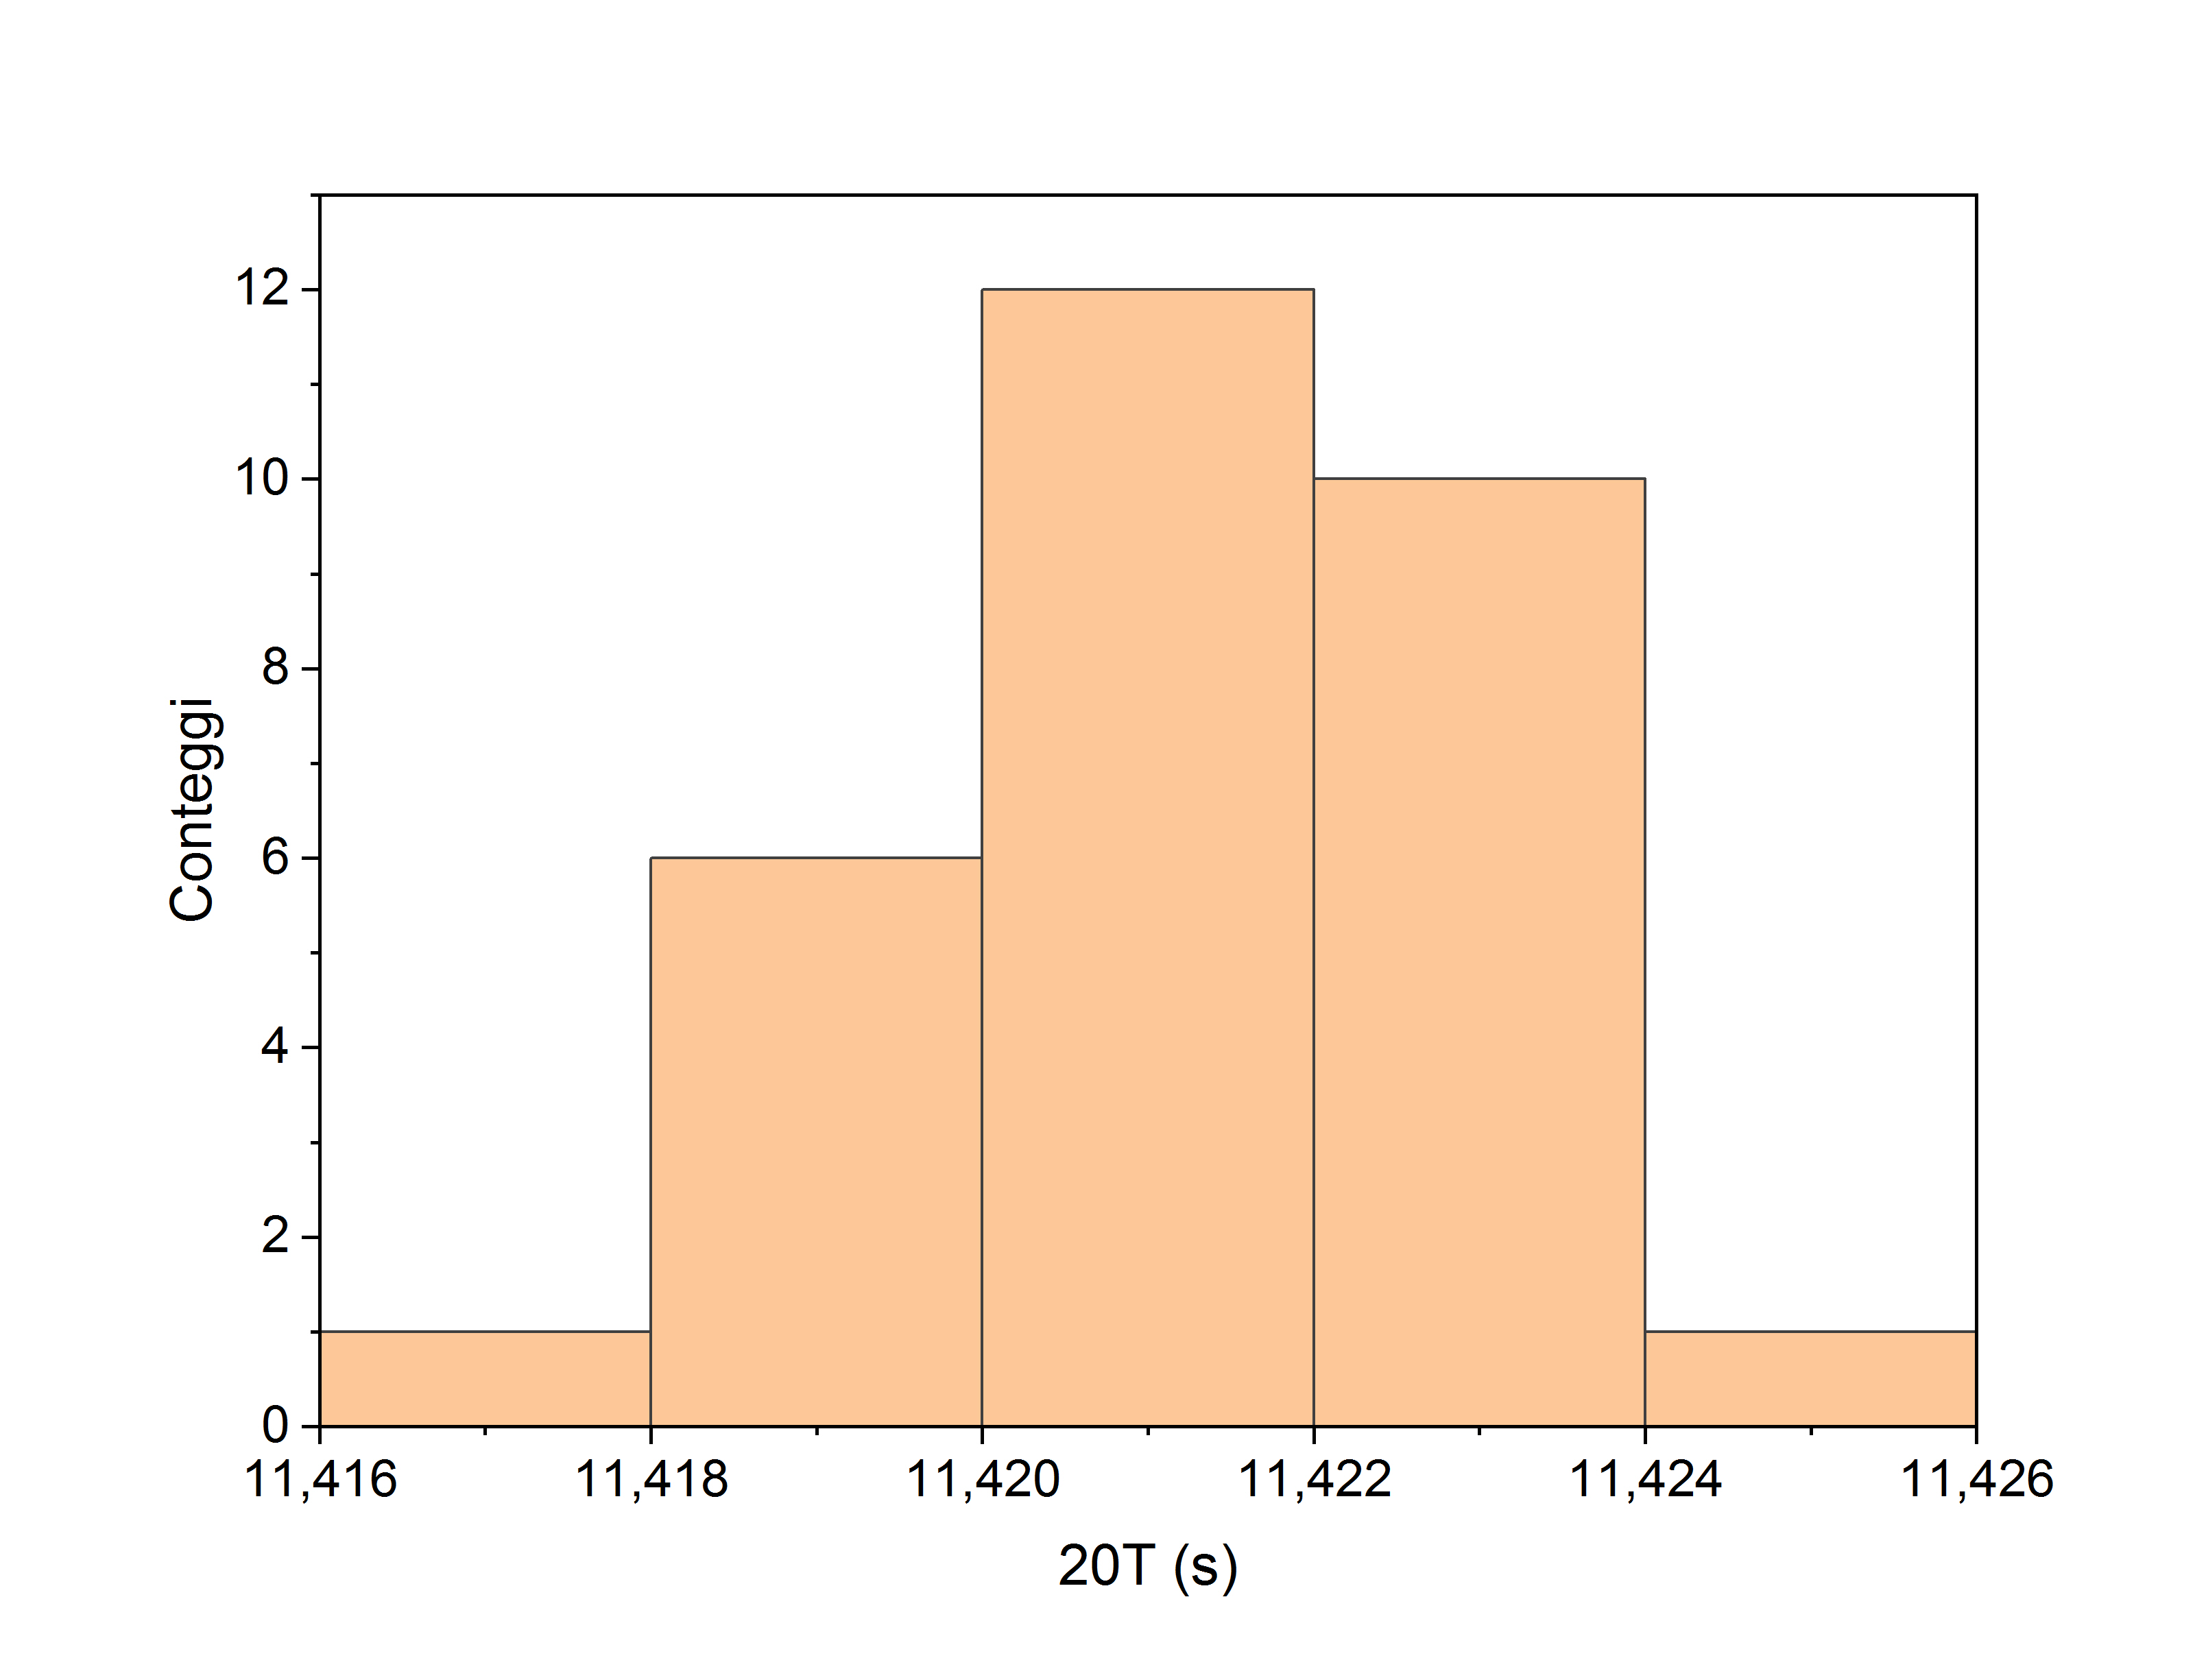
\includegraphics[trim={2cm 1.8cm .7cm 1.5cm},width=.5\textwidth]{Dinamico3.jpg}
    %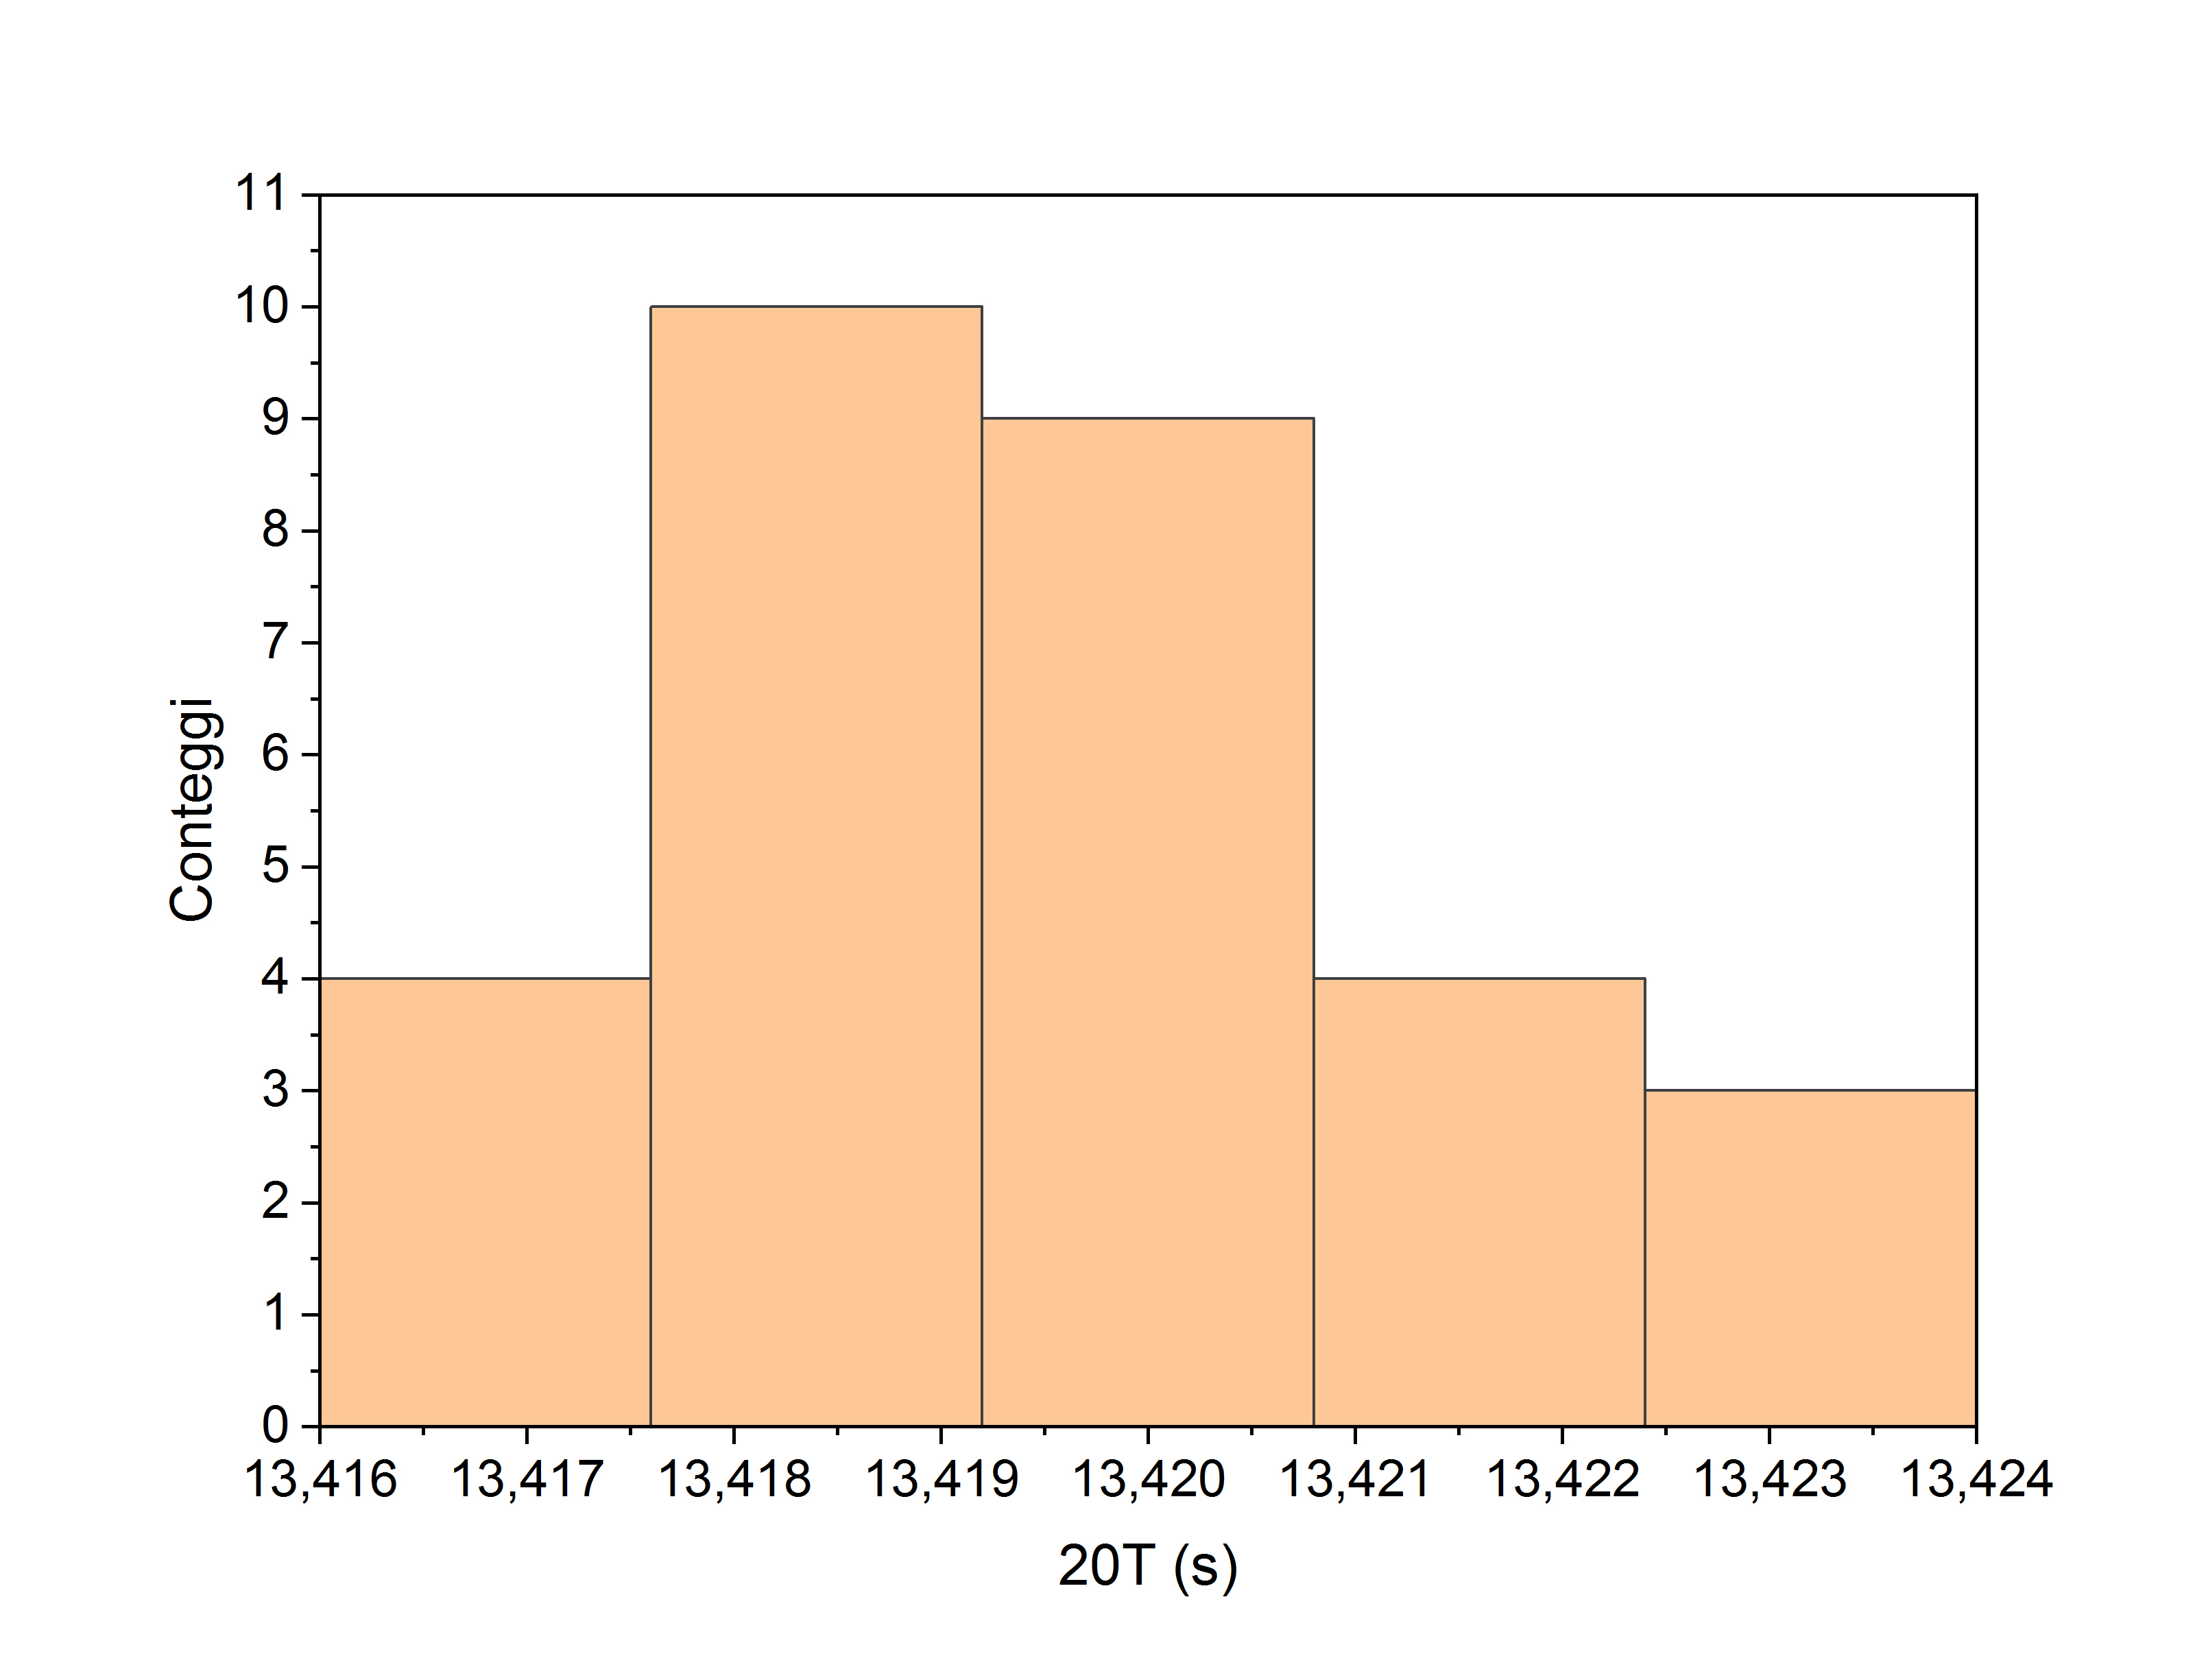
\includegraphics[trim={.7cm 1.8cm 2cm 1.5cm},width=.5\textwidth]{Dinamico4.jpg}
    \caption{Istogrammi dei periodi delle oscillazioni di $C$ e $A+B$}
\end{figure}

Poiché i nostri dati hanno assunto distribuzioni grossolanamente
approssimabili a gaussiane, possiamo procedere al calcolo di $k$,
utilizzando, per ogni grave $i$, i seguenti valori:
\[
    \left(20T_i\right)_\text{best} = \overline{20T_i}
    \qquad\wedge\qquad
    \delta\left(20T_i\right) =
    \sigma_{\overline{20T_i}} =
    \frac{\sigma_{20T_i}}{\sqrt{N_{20T_i}}}
\]
dove $\overline{20T_i}$ e $\sigma_{20T_i}$ indicano rispettivamente
media e deviazione standard dei tempi.

Per determinare la costante elastica della molla, abbiamo effettuato
una regressione lineare (stavolta pesata) sui quadrati dei valori medi
dei tempi ($T_i^2$, con
$\delta T_i^2 = 5 \cdot 10^{-3} (20 T_i)_\text{best} \delta(20 T_i)$
)\footnote[2]{
    La formula per l'errore su $T_i^2$ segue direttamente dalla
    propagazione degli errori:
    \[
        \frac{\delta T_i^2}{\left(T_i^2\right)_\text{best}} = 2\frac{\delta T_i}{{\left(T_i\right)}_\text{best}}
        \qquad
        \delta T_i^2 = 2\left(T_i\right)_\text{best}\delta T_i
        \qquad
        \delta T_i^2 = \frac{\left(20T_i\right)_\text{best}(\delta 20T_i)}{200}
    \]
    da cui quanto riportato sopra.
    Si osservi che $\delta T_i^2$ dipende da
    $\left(20T_i\right)_\text{best}$:
    proprio questo è il motivo dietro alla scelta del metodo pesato
    per la regressione lineare.
} rispetto alla massa $\left(m_\text{eff}\right)_i$, facendo riferimento
alla relazione $T_i^2 = \frac{4\pi^2}{k} \left(m_\text{eff}\right)_i$. Allora, detto $b$ il
coefficiente angolare della retta di regressione, varrà:
\[
    k_\text{best}=\frac{4\pi^2}{b_\text{best}}
    \qquad\wedge\qquad
    \frac{\delta k}{k_\text{best}}=\frac{\delta b}{b_\text{best}}
\]
Si noti che, anche in questo caso, l'intercetta $a$ della retta dev'essere
compatibile con $0$.

Di seguito è riportata la retta di regressione, assieme ai risultati ottenuti:

\begin{figure}[H]
    %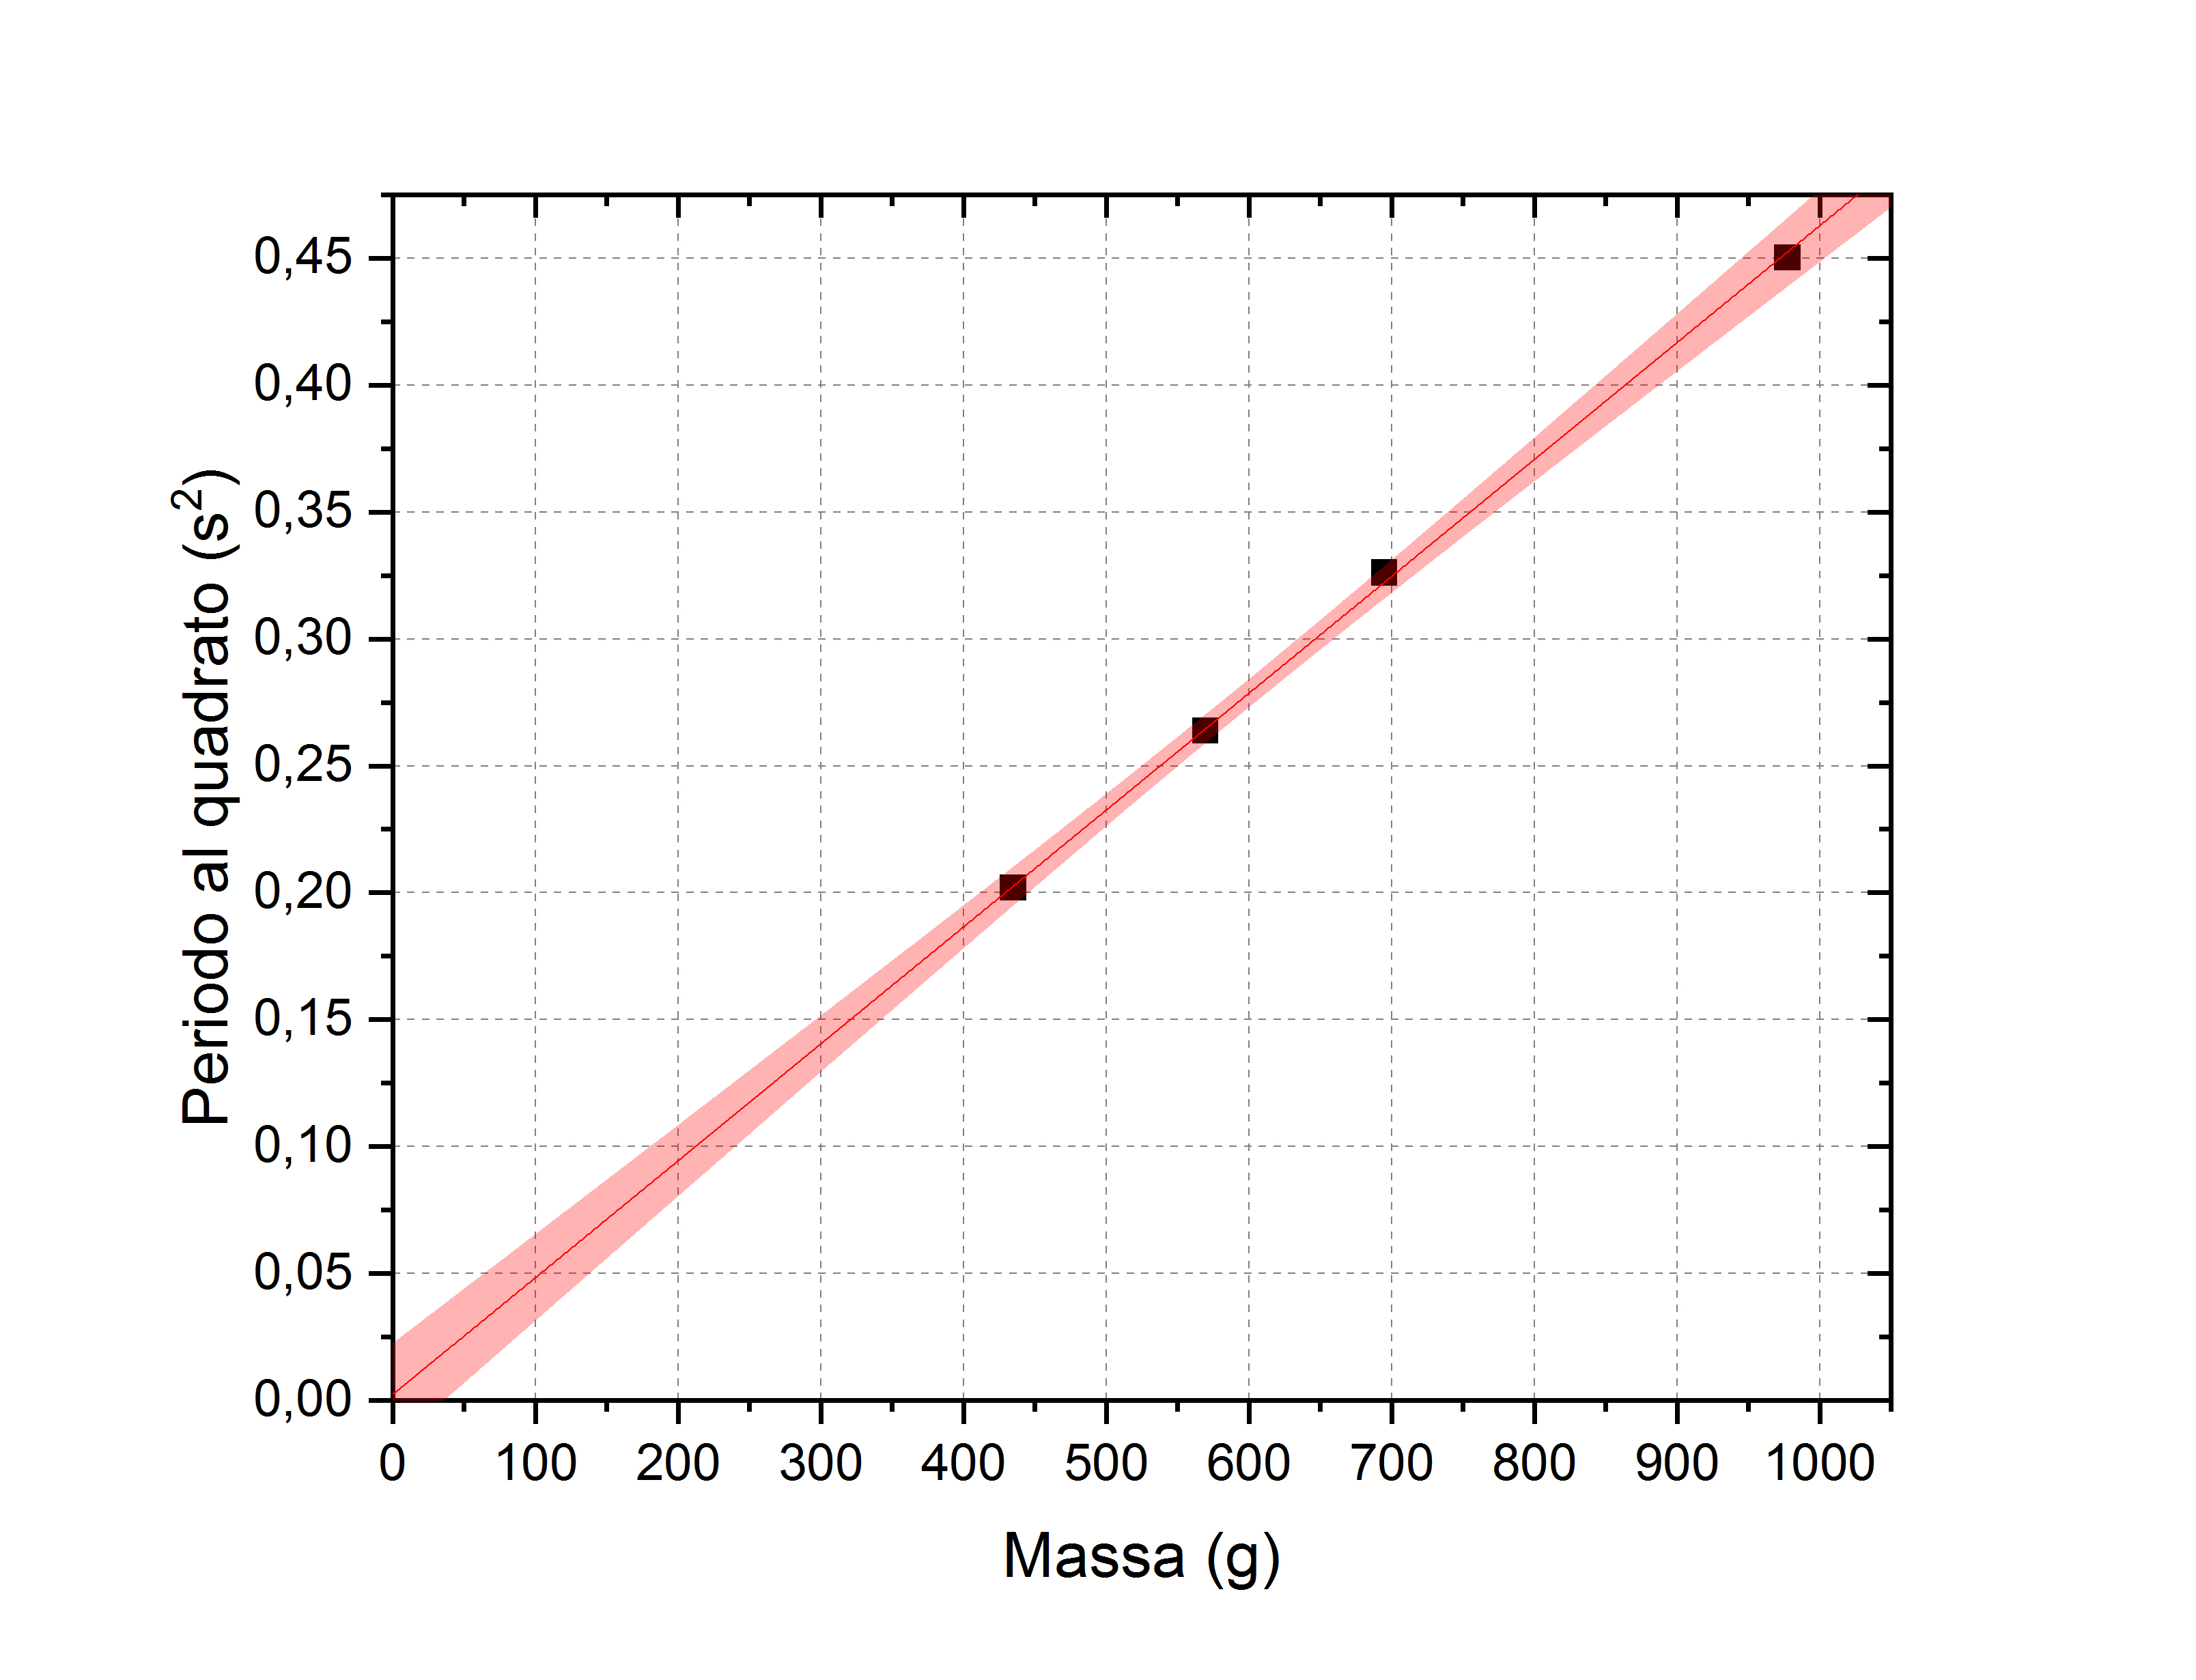
\includegraphics[trim={0 1.8cm 0 0},width=\textwidth]{DinamicoReg.jpg}
    \caption{
        La retta di regressione (in rosso)
        e la sua regione di incertezza (in rosa).
    }
\end{figure}

\begin{itemize}
    \item $a = \left(0.02\pm0.19\right)\unit{cm}$ (compatibile con 0)
    \item $
        b = \left(4.604\pm0.002\right)\cdot10^{-4}\;\unit{s^2\per g}
          = \left(46.04\pm0.02\right)\cdot10^{-2}\;\unit{s^2\per kg}
    $
    \item $k = \left(85.74\pm0.04\right)\unit{N\per m}$
\end{itemize}


\section{Conclusioni}
Per valutare numericamente la consistenza tra i due valori di $k$ ottenuti,
abbiamo calcolato il seguente valore (numero puro):
\[
    \varepsilon =
    \frac{
        \left|\left(k_\text{statica}\right)_\text{best} - \left(k_\text{dinamica}\right)_\text{best}\right|
    }{
        \delta k_\text{statica} + \delta k_\text{dinamica}
    }
\]
Allora $k_\text{statica}$ e $k_\text{dinamica}$ sono consistenti se e solo se $\varepsilon \le 1$.

Nel nostro caso, $\varepsilon = 1.33$. Il gruppo di lavoro ha ipotizzato che
questa inconsistenza (comunque contenuta, seppur non trascurabile) fra le due
misure possa essere ragionevolmente giustificata dalla difficoltà incontrata
nel ridurre al minimo le oscillazioni in direzione perpendicolare a $\vec{g}$;
considerato inoltre che la posizione dei fototraguardi non era ottimale, ciò
potrebbe avere ulteriormente influenzato la distribuzione dei tempi. È in
effetti possibile osservare che le distribuzioni da noi ottenute non sono,
il più delle volte, del tutto simmetriche: la moda sembra essersi spostata
leggermente a sinistra – un possibile sintomo dell'influenza di un
errore sistematico sulle misure.

\end{document}
